\section{Módulo Administrador principal}

  \paragraph{}El diagrama de la figura
  \ref{diagramaDescomposicionAdministradorPrincipal} representa el módulo
  Administrador principal. En primer lugar, el usuario administrador principal
  debe validar sus datos de acceso para que se permita o no el acceso a las
  funciones de las que se compone el módulo.

  \paragraph{}Desde este módulo, el administrador principal podrá acceder a
  todos los procesos necesarios para organizar correctamente toda la estructura
  de la que se compone la aplicación, así como la gestión de copias de seguridad
  de la información que en ella aparezca.

  \paragraph{}Además cuenta con un módulo de ayuda disponible en todo momento
  para el correcto manejo de la aplicación.

  \begin{figure}[!ht]
    \begin{center}
      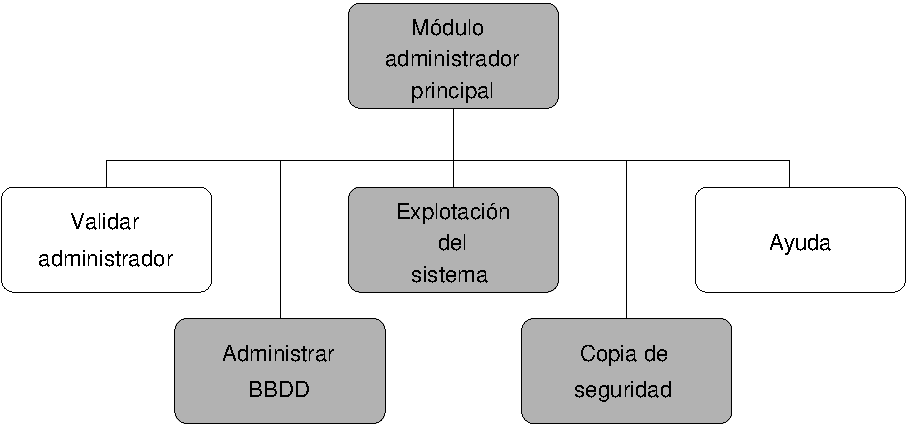
\includegraphics[]{11.Disenyo_Arquitectonico/11.2.Diagramas_Descomposicion/11.2.2.Modulo_administrador_principal/Diagramas/administrador_principal.pdf}
      \caption{Diagrama de descomposición del módulo Administrador principal.}
      \label{diagramaDescomposicionAdministradorPrincipal}
    \end{center}
  \end{figure}

\paragraph{}El usuario administrador principal puede gestionar centros,
departamentos, titulaciones, asignaturas, asesores, alumnos y plantilas
oficiales de la base de datos.

\paragraph{}La figura \ref{diagramaNivel3-AdministrarBBDD-adminPrincipal}
muestra el nivel de abstracción 3: Administrar BBDD (módulo Administrador
principal).

  \begin{figure}[!ht]
    \begin{center}
      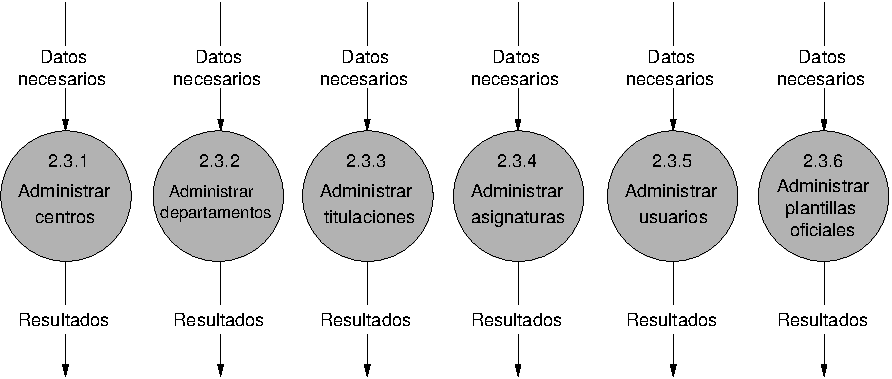
\includegraphics[]{08.Analisis_Funcional/8.2.DFDs/Niveles/Nivel3/AdministradorPrincipal/AdministrarBBDD/Diagramas/nivel3-AdministrarBBDD.pdf}
      \caption{Nivel de abstracción 3: Administrar BBDD (módulo Administrador
      principal).}
      \label{diagramaNivel3-AdministrarBBDD-adminPrincipal}
    \end{center}
  \end{figure}
